\section{Memory Management and Flow Control}
\label{sec:memory}

\begin{table}
  \centering
  \caption{\label{fig:memory-allocator-compare} A comparison of Themis's memory
    allocator implementations.}
  \tabcolsep=0.11cm

  \begin{tabular}{|c|c|c|p{.7cm}|p{.7cm}|p{.7cm}|c|} \hline
    & \multirow{2}{*}{\textbf{TritonSort}} & \multirow{2}{*}{\textbf{Themis}}
    & \multicolumn{3}{c|}{\textbf{Used in Phase}} & \textbf{Subject to} \\\cline{4-6}
    & & & \centering 0 & \centering 1 & \centering 2 & \textbf{deadlock?} \\ \hline
    Pool & $\checkmark$ & $\checkmark$ & \centering $\checkmark$ & \centering $\checkmark$ & & \\\hline
    Quota &  & $\checkmark$ & \centering $\checkmark$ & \centering $\checkmark$ & &  \\\hline
    Constraint &  & $\checkmark$ &  &  & \centering $\checkmark$ & $\checkmark$ \\\hline
  \end{tabular}
\end{table}

Themis relies on a dynamic and flexible memory management system
to partition memory between operators.
Themis's memory manager actually serves two distinct purposes: (1) it
enables resource sharing between operators, and (2) it supports
enforcing back-pressure and flow control.  In the first case, Themis requires
flexible use of memory given our desire to support large amounts of record
size
skew while maintaining the 2-IO property.  In the second case, individual
stages in the Themis pipeline naturally run at different speeds (e.g.,
the network is 10 Gbps, whereas the disk subsystem only supports writing
at approximately 5.5 Gbps), and so back-pressure and flow control are needed
to prevent faster stages from starving slower stages for resources.

Themis supports a single memory allocation interface with pluggable memory
policies.  We first describe the memory allocator's interface, and then
describe the three policies that we have implemented.

\subsection{Memory Allocation Interface}

Worker stages in Themis allocate space for buffers and other necessary
scratch space using a unified and simple memory allocator interface,
shown in Table~\ref{fig:memory-allocator-API}.

\begin{table*}
  \centering
  \caption{\label{fig:memory-allocator-API} A summary of the Themis memory
    allocator API.}
  \resizebox{\columnwidth}{!}{
  \begin{tabular}{|l|l|}
    \hline
    \textbf{Function} & \textbf{Description} \\
    \hline
    \texttt{CallerID \textbf{registerCaller}(Worker worker)} & Register \texttt{worker}
    with the allocator \\
    \hline
    \texttt{void* \textbf{allocate}(CallerID caller, uint64\_t size)} & allocate a
    memory region of \texttt{size} bytes for \texttt{caller} \\
    \hline
    \texttt{void \textbf{deallocate}(void* memory)} & deallocate \texttt{memory} that
    was allocated by this allocator\\
    \hline
  \end{tabular}
  }
\end{table*}

Memory allocators can be assigned on a stage-by-stage basis, but in the current
implementation we assume that memory regions are allocated and deallocated by
the same allocator.  The \texttt{allocate} call blocks until the underlying
memory allocation policy satisfies the allocation, which can be an unbounded
amount of time.  As we will see, this simple mechanism, paired with one of
three memory policies, provides for both resource sharing as well as flow
control.  We now examine each of these polices.

\subsection{Policy 1: Pool-Based Management}

\begin{figure}
  \centering
  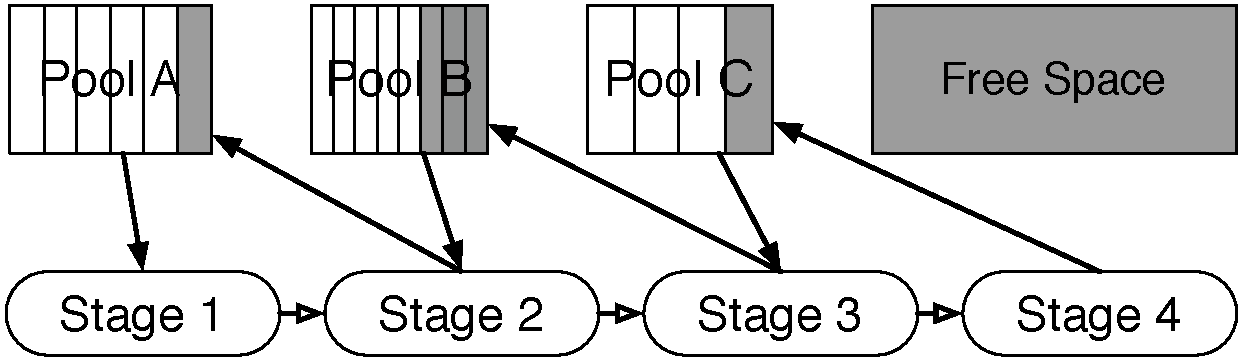
\includegraphics[width=\columnwidth]{themis/figures/pool_based_manager.pdf}
  \caption{\label{fig:memory_allocators:pool} A diagrammatic overview of
    pool-based memory management. Note that memory in each pool is divided into
  fixed-size regions, and that any memory not allocated to pools cannot be
  utilized by stages.}
\end{figure}

The first policy we consider is a ``pool'' memory policy, which is inherited
from TritonSort~\cite{tritonsort}.  A memory pool is a set of pre-allocated
buffers that is filled during startup.  Buffers can be checked out from a pool,
and returned when they are finished being used as illustrated in
Figure~\ref{fig:memory_allocators:pool}.  When a worker tries to check out a
buffer from an empty pool, it blocks until another worker returns a buffer to
that pool.  The pool memory policy has the advantage that all memory allocation
is done at startup, avoiding allocation during runtime.  Through efficient
implementation, the overhead of checking out buffers can be very small.  This
is especially useful for stages that require obtaining buffers with very low
latency, such as the \Receiver stage, which obtains buffers to use in receiving
data from the network.  The \receiver receives uninterpreted bytes from network
sockets into small, fixed-size byte buffers.  These buffers are passed to a
subsequent stage, which converts them into buffers containing complete records.
For this reason, the \receiver can use pool-based management while still
supporting record-size skew.

Pools can be used to provide resource sharing between workers by giving each of
those workers a reference to a single pool.  The producer-consumer relationship
between pairs of stages also provides a form of flow control; the upstream
stage checking out buffers can only produce work at the rate at which the
downstream stage can return them to the pool.  However, pools have several
disadvantages.  First, the buffers in a pool are all fixed-size, and so
the pool memory policy supports very limited amounts of data skew.  By
carving memory up into fixed-size pools, the maximum record size supported by
this policy is limited to the size of the smallest pool.  Additionally, buffer
pools reserve a fixed amount of memory for a particular pair of stages. One
consequence of this is a loss of flexibility; if one stage temporarily needs
more memory than usual (e.g., if it is handling a large record), it cannot
``borrow'' that memory from another stage due to the static partitioning of
memory across pools.

\subsection{Policy 2: Quota-Based Management}

\begin{figure}
  \centering
  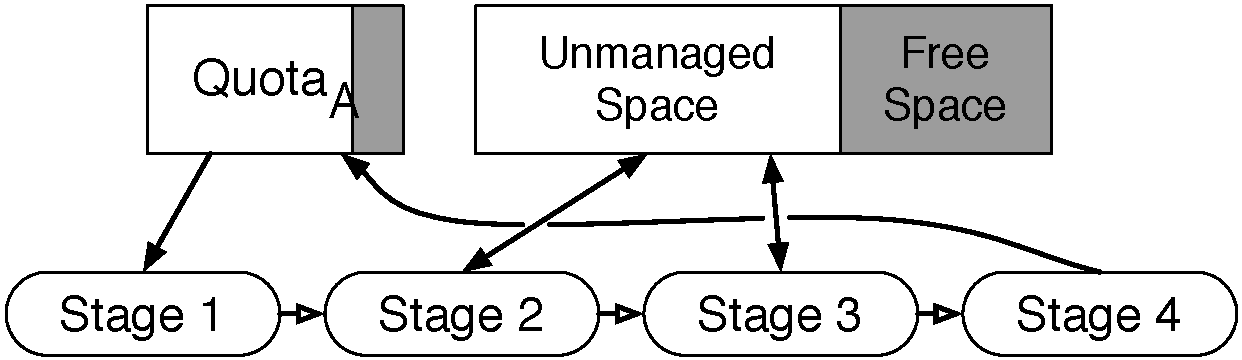
\includegraphics[width=\columnwidth]{themis/figures/quota_based_manager.pdf}
  \caption{\label{fig:memory_allocators:quota} A diagrammatic overview of
    quota-based memory management. In this figure, $Quota_A$ provides a memory
    quota between Stage 1 and Stage 4. Stages 2 and 3 use unmanaged memory
    created with standard \texttt{malloc} and \texttt{free} syscalls.}
\end{figure}

While the pool memory policy is simple, it is quite inflexible, and does not
handle skewed record sizes very well.  The quota-based memory policy is
designed to support more flexible memory allocation while still providing flow
control.  At a high level, the quota policy ensures that stages producing
records do not overwhelm stages that eventually consume them.  For example,
most of our evaluation is \writer limited, and so we want to ensure that the
\receiver stage, which produces records received from the network, does not
overwhelm the \writer stage, which is the bottleneck.

Themis has three such producer-consumer pairs: between the \reader and the
\mapper (with the \mapper acting as the consumer), between the \mapper and the
\sender (with the \mapper acting as the producer), and between the \receiver
and the \writer. The mapper acts as both a consumer and a producer, since it is
the only stage in the phase one pipeline that creates records as directed by
the \map function that were not read by the \reader.

Quotas are enforced by the queues between stages. A quota can be viewed as the
amount of memory that the pipeline between a producer and a consumer can use.
When a producer stage pushes a buffer into the pipeline, the size of that
buffer is debited from the quota.  When a consumer stage consumes that buffer,
the buffer's size is added back to the quota.  If a producer is about to exceed
the quota, then it blocks until the consumer has consumed sufficient
memory. Quota-based allocation is illustrated in
Figure~\ref{fig:memory_allocators:quota}.

Quota-based memory management dramatically reduces the number of variables that
need to be tuned relative to the pool-based memory policy.  One need only
adjust the quota allocations present between pairs of stages, rather than the
capacity of a much larger number of buffer pools.  Additionally, stages that
are not producers and consumers do not need to do any form of coordination,
which makes their memory allocations very fast.

Quota-based management assumes that any scratch space or additional memory
needed by stages between the producer and consumer is accounted for in the
quota.  This is to prevent intermediate stages from exceeding the total amount
of memory, since their memory accesses are not tracked.  It also tacitly
assumes that the size of a buffer being produced cannot exceed the size of the
quota. This is much less restrictive than a pool-based approach, as quotas are
typically several gigabytes.

\subsection{Policy 3: Constraint-Based Management}

\begin{figure}
  \centering
  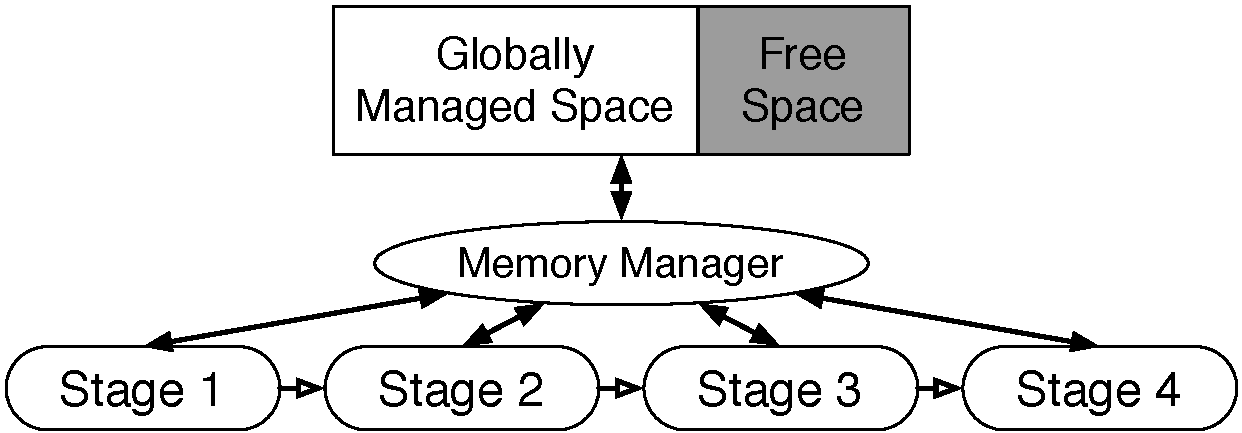
\includegraphics[width=\columnwidth]{themis/figures/constraint_based_manager.pdf}
  \caption{\label{fig:memory_allocators:constraint} A diagrammatic overview of
    constraint-based memory management. All stages' memory requests are
    satisfied by a central memory manager that schedules these requests
    according to the stage graph's structure.}
\end{figure}

In situations where the amount of memory used by stages to process records
cannot be determined in advance, quota-based systems are not ideal for
providing flow control. In these situations, Themis uses a more heavyweight,
constraint-based memory management policy.

In the constraint-based memory policy, the total amount of memory in use by
workers is tracked centrally in the memory allocator. If a worker requests
memory, and enough memory is available, that request is granted immediately.
Otherwise, the worker's request is added to a per-worker queue of outstanding
requests and the worker sleeps on a condition variable until the request can be
satisfied. Constraint-based allocation is illustrated in
Figure~\ref{fig:memory_allocators:constraint}.

When multiple workers have outstanding unsatisfied allocation requests, the
memory allocator prioritizes worker requests based on a worker's distance in
the stage graph to a stage that consumes records.  The producer-side pipeline
measures distance to the \sender stage, and the consumer-side pipeline measures
distance to the \writer stage.  The rationale behind this decision is that
records that are being processed should be completely processed before more
work is admitted. This decision is inspired by work on live-lock prevention in
routers~\cite{ReceiveLivelock}.  In this way, the constraint-based allocator
implements flow control based on the structure of the dataflow graph.

While this system places precise upper bounds on the amount of memory present
in the system, it requires a great deal of coordination between workers, which
requires significant lock contention in our implementation.  In effect, the
reliance on keeping the amount of available memory consistent requires that all
allocation and deallocation requests are processed serially. Hence,
constraint-based memory allocation is useful for situations where the number of
allocation requests being made is relatively small, but the probability of
exceeding available memory in common-case operation is high.  Phase two in
Themis uses constraint-based memory management for precisely these reasons.

In the constraint-based policy, it is possible that certain allocation
interleavings can trigger deadlock.  Predicting whether a general dataflow
system will deadlock is undecidable~\cite{NajjarLeeGao}, and deadlock
prevention requires knowledge of data dependencies between stages that we
deemed too heavyweight. To addressed the problem of deadlocks, Themis provides
a deadlock detector. The deadlock detector periodically probes workers to see
if they are waiting for a memory allocation request to complete. If multiple
probe cycles pass in which all workers are waiting for an allocation or are
idle, the deadlock detector informs the memory allocator that a
deadlock has occurred.  We have not experienced deadlock using the policy
choices described in Table~\ref{fig:memory-allocator-compare} in any of the
MapReduce jobs we have evaluated.  Efficient ways of handling deadlock is the
subject of ongoing work.

In summary, Themis provides a pluggable, policy-driven memory allocation
subsystem that provides for flexible resource sharing between stages and
workers to handle record size skew while also enabling flow control.
% LocalWords:  livelock TritonSort's demux
